\chapter{Connecting and Breakout Board Schematic}\label{app:ConnectingBreakoutBoard} 

The connecting and breakout board present in the system has been done by Simon Jensen, Electronic Technician at Aalborg University.

\subsection{Input and Output Connections}
The BeagleBone Black input and output connections diagram \figref{labExpanionHeader}:\\
\begin{figure}[H]
	\centering
	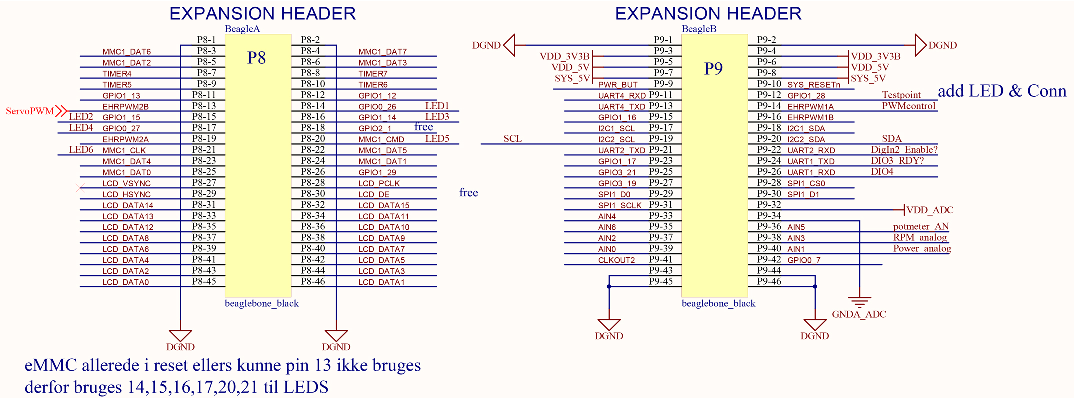
\includegraphics[scale=0.92]{figures/ExpanionHeader.pdf}
	\caption{Expansion header diagram.}
	\label{labExpanionHeader}
\end{figure}\vspace{-5mm}
%Schematic of the Connecting and Breakout Board.

\subsection{Voltage Information}
The power supply that supplies the entire system is 24 V. There has been built voltage regulators in to the connecting and breakout board to supply the different units with operation voltage. Many connections between the different units and the BeagleBone Black has to be in the same voltage level, for the BeagleBone Black to be compatible with the units.

Many of the sensors are operating on different voltage. Below is a list of the different voltage usage:
\begin{table}[H]
	\begin{tabular}{|l|l|p{4.3cm}|}
		\hline%------------------------------------------------------------------------------------------------------------
		\textbf{Unit}       &  \textbf{Voltage (V)}         \\
		\hline%------------------------------------------------------------------------------------------------------------
		BeagleBone Black                               & 5 V           \\
		\hline%------------------------------------------------------------------------------------------------------------
		BeagleBone Black ADC							  & Max. 1,8 V              \\
		\hline%------------------------------------------------------------------------------------------------------------
		BeagleBone Black logic level							  & 3,3 V              \\
		\hline%------------------------------------------------------------------------------------------------------------
		Maxon Controller Board 							  & 10 V to 50 V              \\
		\hline%------------------------------------------------------------------------------------------------------------
		Maxon Motor							  & 24 V             \\
		\hline%------------------------------------------------------------------------------------------------------------
		Potentiometer							  & Max. 50 V              \\
		\hline%------------------------------------------------------------------------------------------------------------
		ServoMotor							  & 4,8 V to 6 V              \\
		\hline%------------------------------------------------------------------------------------------------------------
		IMU PMU6050							  & 3,3 V              \\
		\hline%------------------------------------------------------------------------------------------------------------
	\end{tabular}
\end{table}

\subsection{Potentiometer Connections}
The Potentiometer connections diagram \figref{labPotmeter}:\\

\begin{figure}[H]
	\centering
	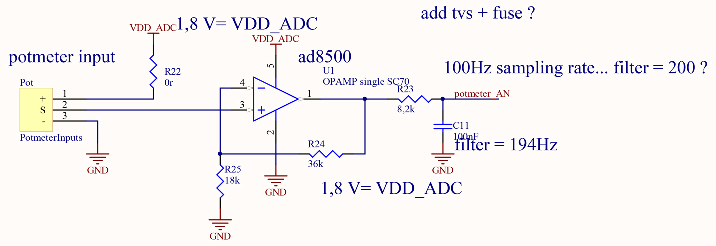
\includegraphics[scale=0.92]{figures/Potmeter.pdf}
	\caption{Potentiometer diagram.}
	\label{labPotmeter}
\end{figure}\vspace{-5mm}

The Potentiometer is connected to the BeagleBone’s A/D and only a small area is used on the Potentiometer, and for this reason the signal is gained and it is done by using an Operational Amplifiers (op-amp) which can only gain the voltage to 1,8 V, because of the supply voltage to the op-amp is only 1,8 V.

The Potentiometer is only using a small area of rotation on the Cubli, about ¼ of the full rotation. The gain is calculated from the max. rotation voltage and the result is a gain of 3 V. 

To verify the gain, the potentiometer voltage is measured and the ADC value is read from the BeagleBone Black.
\begin{table}[H]
	\begin{tabular}{|l|l|p{4.3cm}|}
		\hline%------------------------------------------------------------------------------------------------------------
		\textbf{Unit}       &  \textbf{Voltage (V)}         \\
		\hline%------------------------------------------------------------------------------------------------------------
		Measured before the gain                               & 0,470 V           \\
		\hline%------------------------------------------------------------------------------------------------------------
		0,470 V with a gain of 3							  & 1,410 V              \\
		\hline%------------------------------------------------------------------------------------------------------------
		Measured after the gain							  & 1,417 V              \\
		\hline%------------------------------------------------------------------------------------------------------------
		ADC value  							  & 1,419              \\
		\hline%------------------------------------------------------------------------------------------------------------
	\end{tabular}
\end{table}
After the signal has been gained, a low-pass filter with a frequency of 194 Hz is added to damp noise on the signal. 
%Since the sampling frequency is 100 Hz it is almost upholding New Quest by double or faster

\subsection{Motor Control Board Connections}
The Maxon Motor Driver Board connections diagram \figref{labMotorDriver}:\\

\begin{figure}[H]
	\centering
	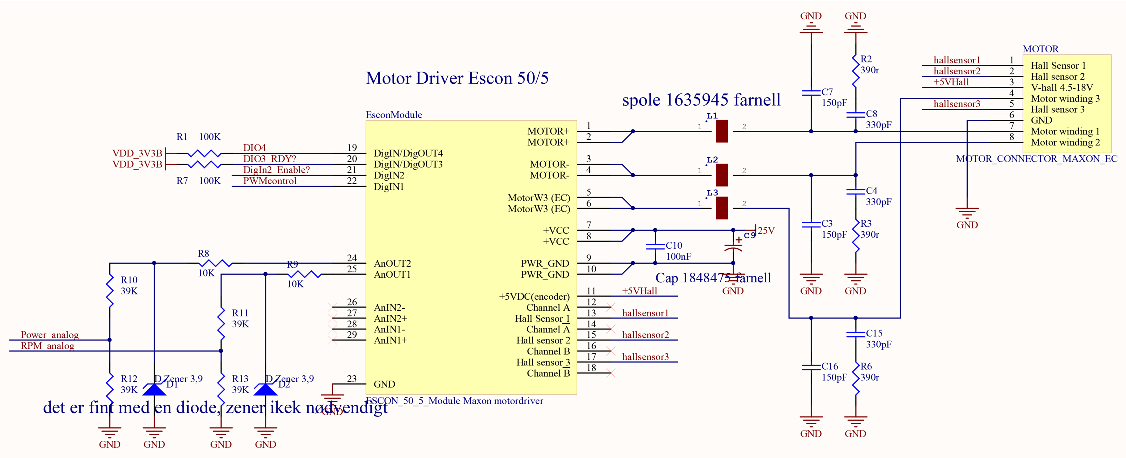
\includegraphics[scale=0.92]{figures/MotorDriver.pdf}
	\caption{Motor Driver diagram.}
	\label{labMotorDriver}
\end{figure}\vspace{-5mm}

Since the BeagleBone Black ADC only operates up to \SI{1,8}{V} and the Maxon control board operates at \SI{-4}{V} to \SI{4}{V}, a voltage divider has been put in from the Maxon motor control to the Beagle Bone so the BeagleBone’s A/D limit is not exceeded so the voltage is multiplied by 0,44382. Then if the Maxon controller operates at a maximum of \SI{4}{V} it becomes \SI{1,77528}{V} below the BeagleBone A/D limit of \SI{1,8}{V}.

\subsection{Extra Connections}
MPU6050's I2C and \SI{3,3}{V} connections to the BeagleBone Black.
\begin{figure}[H]
	\centering
	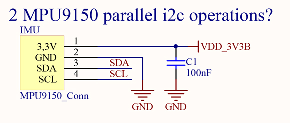
\includegraphics[scale=0.92]{figures/PMU9150.pdf}
	\caption{PMU6050 connections diagram.}
	\label{labPMU9150}
\end{figure}\vspace{-5mm}

\SI{5}{V} power supply for the ServoMotor on Connecting and Breakout Board, and \SI{3,3}{V} to \SI{5}{V} level converter is needed to get the BeagleBone Black PWM signals to the ServoMotors logic circuit. 
\begin{figure}[H]
	\centering
	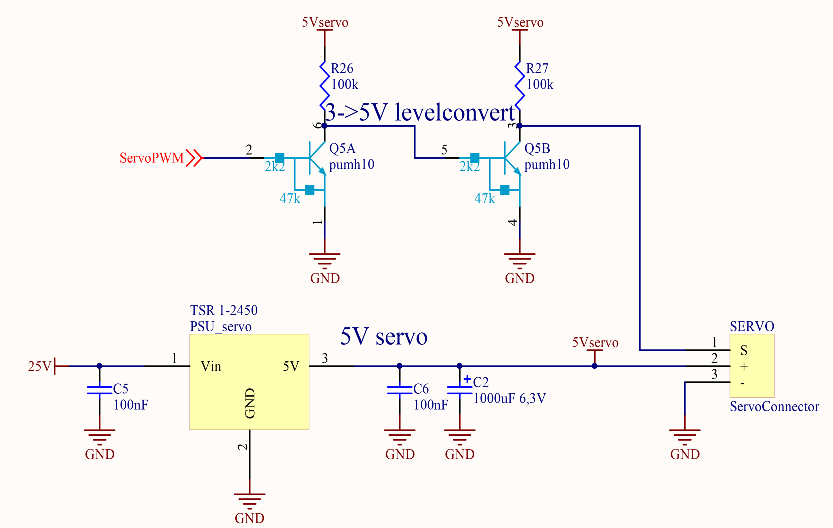
\includegraphics[scale=0.92]{figures/ServoMotor.pdf}
	\caption{ServoMotor diagram.}
	\label{labServoMotor}
\end{figure}\vspace{-5mm}

\SI{5}V power supply for the BeagleBone Black and the LED’s on Connecting and Breakout Board.
\begin{figure}[H]
	\centering
	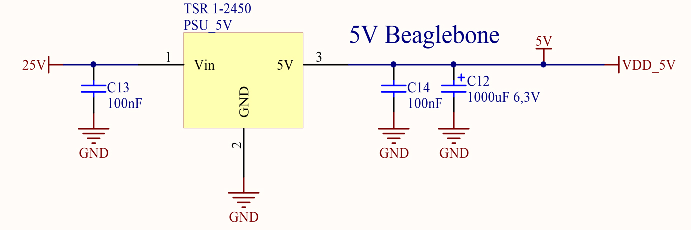
\includegraphics[scale=0.92]{figures/BeagleBone.pdf}
	\caption{Power converter from \SI{25}{V} to \SI{5}{V} for the BeagleBone Black.}
	\label{labBeagleBone}
\end{figure}\vspace{-5mm}

\SI{25}{V} power and grounding connections and \SI{5}{V} and \SI{3,3}{V} LED's connections.
\begin{figure}[H]
	\centering
	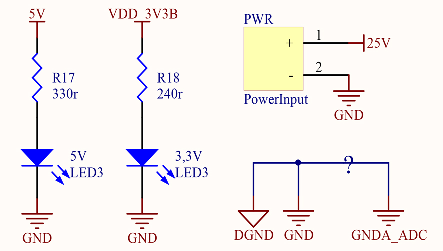
\includegraphics[scale=0.92]{figures/Power.pdf}
	\caption{Power diagram.}
	\label{labPower}
\end{figure}\vspace{-5mm}

\SI{5}{V} LED's connections to the BeagleBone Black.
\begin{figure}[H]
	\centering
	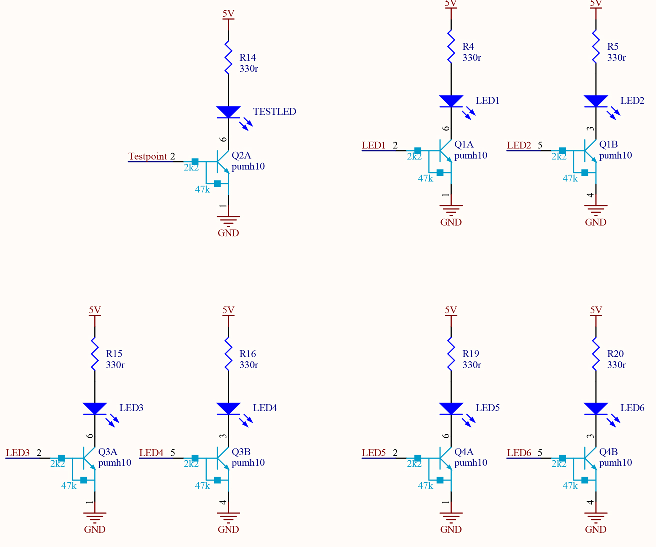
\includegraphics[scale=0.92]{figures/Led.pdf}
	\caption{LED's diagram to the BeagleBone Black.}
	\label{labLed}
\end{figure}\vspace{-5mm}


%
%\subsubsection{List of Equipment}
%\begin{table}[H]
%	\begin{tabular}{|l|l|p{4.3cm}|}
%		\hline%------------------------------------------------------------------------------------------------------------
%		\textbf{Instrument}                                  &  \textbf{AAU-no.}  &  \textbf{Type}                       \\
%		\hline%------------------------------------------------------------------------------------------------------------
%		Multimeter                                           &  60760           &  Fluke 189 Multimeter		                   \\
%		\hline%------------------------------------------------------------------------------------------------------------
%		Dedicated Power Supply of Cubli \small{(24 V - 3 A)} &  AAU3                   &  XP Power, AEB70US24                 \\
%		\hline%------------------------------------------------------------------------------------------------------------
%		Digital Protractor                                   &  None               & CMT Orange Tools     \\
%		\hline%------------------------------------------------------------------------------------------------------------
%	\end{tabular}
%\end{table}
%
%\subsubsection{Procedure}
%\begin{enumerate}
%  \item The Cubli base frame is leveled and the angle of equilibrium point is measured.
%  \item The frame is dismounted from the base frame and weight.
%  \item The frame is mounted back on the base frame after been rotated 90 degrees and the angle of equilibrium point is measured.
%  \item The Cubli frame is returned to original placement on the base frame.
%\end{enumerate}
%
%\subsubsection{Results}
%\begin{table}[H]
%	\begin{tabular}{|l|l|p{4.3cm}|}
%		\hline%------------------------------------------------------------------------------------------------------------
%		\textbf{Frame rotation angle in degrees}       &  \textbf{Angle form equilibrium point in degrees}         \\
%		\hline%------------------------------------------------------------------------------------------------------------
%		0                                & 2,50           \\
%		\hline%------------------------------------------------------------------------------------------------------------
%		90							  & 4,50              \\
%		\hline%------------------------------------------------------------------------------------------------------------
%	\end{tabular}
%\end{table}
%
%\subsubsection{Results}
%\begin{table}[H]
%	\begin{tabular}{|l|l|p{4.3cm}|}
%		\hline%------------------------------------------------------------------------------------------------------------
%		\textbf{Weight of the frame}       &  \textbf{Gram}         \\
%		\hline%------------------------------------------------------------------------------------------------------------
%		 Fully mounted frame        	  & 770          \\
%		\hline%------------------------------------------------------------------------------------------------------------
%	\end{tabular}
%\end{table}	
